\documentclass[compress, aspectratio=54]{beamer}
%\documentclass[notes=show]{beamer}
%\documentclass[xcolor=dvipsnames]{beamer}
\usepackage[export]{adjustbox}
\usepackage{sidecap}
\usepackage{subfig}
\usepackage{amssymb}
\usepackage{latexsym}
\usepackage{amsfonts}
\usepackage{amsmath}
\usepackage[absolute,overlay]{textpos}
\usepackage[english]{babel}
\usepackage[latin1]{inputenc}
\usepackage{subfig}
%\usepackage{times}
\usepackage[T1]{fontenc}
\usepackage{tabularx}
\newcolumntype{Y}{>{\small\raggedright\arraybackslash}X}
\usepackage{graphicx}
\usepackage{bigstrut}
\usepackage{bbm}
\usepackage{mathrsfs}
\usepackage{epsfig}
\usepackage{array}
%\usepackage{natbib}
\usepackage{hyperref}
\usepackage{caption}

\mode<presentation> {
%\usetheme[left,width=1.7cm]{Berkeley}
%\usetheme{default}
\usetheme{Boadilla}
  \usecolortheme[RGB={103,102,204}]{structure}
%\usecolortheme{dove}
  \useoutertheme{infolines}
  \setbeamercovered{transparent}
 }

%\usepackage[utf8]{inputenc}

% Default fixed font does not support bold face
\DeclareFixedFont{\ttb}{T1}{txtt}{bx}{n}{12} % for bold
\DeclareFixedFont{\ttm}{T1}{txtt}{m}{n}{12}  % for normal

% Custom colors
\usepackage{color}
\definecolor{deepblue}{rgb}{0,0,0.5}
\definecolor{deepred}{rgb}{0.6,0,0}
\definecolor{deepgreen}{rgb}{0,0.5,0}

\usepackage{listings}

% Python style for highlighting
\newcommand\pythonstyle{\lstset{
language=Python,
basicstyle=\ttm,
otherkeywords={self},             % Add keywords here
keywordstyle=\ttb\color{deepblue},
emph={MyClass,__init__},          % Custom highlighting
emphstyle=\ttb\color{deepred},    % Custom highlighting style
stringstyle=\color{deepgreen},
frame=tb,                         % Any extra options here
showstringspaces=false            % 
}}


% Python environment
\lstnewenvironment{python}[1][]
{
\pythonstyle
\lstset{#1}
}
{}

% Python for external files
\newcommand\pythonexternal[2][]{{
\pythonstyle
\lstinputlisting[#1]{#2}}}

% Python for inline
\newcommand\pythoninline[1]{{\pythonstyle\lstinline!#1!}}
%\renewcommand{\familydefault}{cmss}
%\renewcommand{\mathrm}{\mathsf}
%\renewcommand{\textrm}{\textsf}
\usefonttheme{serif}
\newcommand{\X}{{\mathbf{X}}}
\newcommand{\x}{{\mathbf{x}}}
\newcommand{\E}{\mathsf{E}}
\newcommand{\V}{\mathsf{Var}}

\DeclareGraphicsExtensions{.jpg,.pdf,.mps,.png}

\setbeamercolor{bibliography entry title}{fg=black}
\setbeamercolor{bibliography entry author}{fg=black}
\setbeamercolor{subsection in toc}{fg=structure}
\setbeamercolor{palette primary}{bg=structure, fg=white}
%\setbeamercolor{palette secondary}{bg=structure, fg=black}
%\setbeamercolor{palette tertiary}{bg=structure, fg=black}
\setbeamercolor{caption name}{fg=black} \setbeamersize{text margin
left=.8cm} \setbeamersize{text margin right=1cm}
\hypersetup{linkbordercolor={1 0 0}} \setbeamertemplate{navigation
symbols}{} \setbeamertemplate{headline}[default]

\setbeamertemplate{enumerate items}[default]

\newcounter{transfct}
\newcounter{begbs}
\newcounter{endbs}


\title[ML for NLP ]{Machine Learning for Natural Language Processing}

\author[Arieda Mu\c co]{Arieda Mu\c co\footnote{based on material from Andreas Mueller (slides and book)}}
\institute[CEU]{Central European University}
\date{ }

\AtBeginSection[] {
  \begin{frame}<handout:0>
    \frametitle{TOC}
    \tableofcontents[currentsection]
  \end{frame}
}


\AtBeginSection[] {
  \begin{frame}<handout:0>
    \frametitle{TOC}
    \tableofcontents[currentsection]
  \end{frame}
}


\pgfdeclareimage[height=.7cm]{logo}{rgs2}
\logo{\pgfuseimage{logo}}
\begin{document}
\captionsetup[subfigure]{labelformat=empty}

\frame{\titlepage}

%%%%%%%%%%%%%%%%%%%%%%%%%%%%%%%%%%%%%%%%%%%

\begin{frame}
\begin{center}
\Large{\textbf{Missing observations}}
\end{center}
\end{frame}

\begin{frame}
\frametitle{Missing Values}
Missing values can be encoded in many ways

\begin{itemize}
\item Numpy has no standard format for it (often np.NaN) 
\item Sometimes you will encounter missing values encoded as: 999 (you can go on adding more "9" here), "???", "?", "np.inf", "N/A", "Unknown", "." ?
\item Often missingness is informative
\begin{itemize}
\item Checking other covariates
\item Code missing as indicator 1 if missing and zero otherwise.
\end{itemize}
\item  If you use variables in the dataset to predict if missing category, make sure your outcome is not one of them. Why? Can you show this?
\end{itemize}

\end{frame}



\begin{frame}
\frametitle{Do }
Understand your data. Some common imputation methods for replacing missing values are
\begin{itemize}
\item Mean or Median -- conditioning for other covariates. Regression models

\item K-nearest neighbours
\begin{itemize}

\item  Find k nearest neighbors that have non-missing values

\item  Fill in all missing values using the average of the neighbors
\end{itemize}
\item Model-Driven Imputation. Train regression model for missing values (retrain model after filling in)


\end{itemize}
\end{frame}


\begin{frame}
\frametitle{Don't}
\begin{itemize}
\item Drop observations with the default drop missings command  (Stata/Python/R...)

\item Start doing analysis without understanding the missings
\begin{itemize}

\item Algorithms don't understand missings and will drop them. You will end up with a selected sample.
\item If your missings are coded as "9999" will skew the data and your results are not valid
\end{itemize}

\end{itemize}
\end{frame}



\begin{frame}
\begin{center}
\Large{\textbf{Cross-Validation}}
\end{center}
\end{frame}

\begin{frame}
\frametitle{}
\begin{figure}

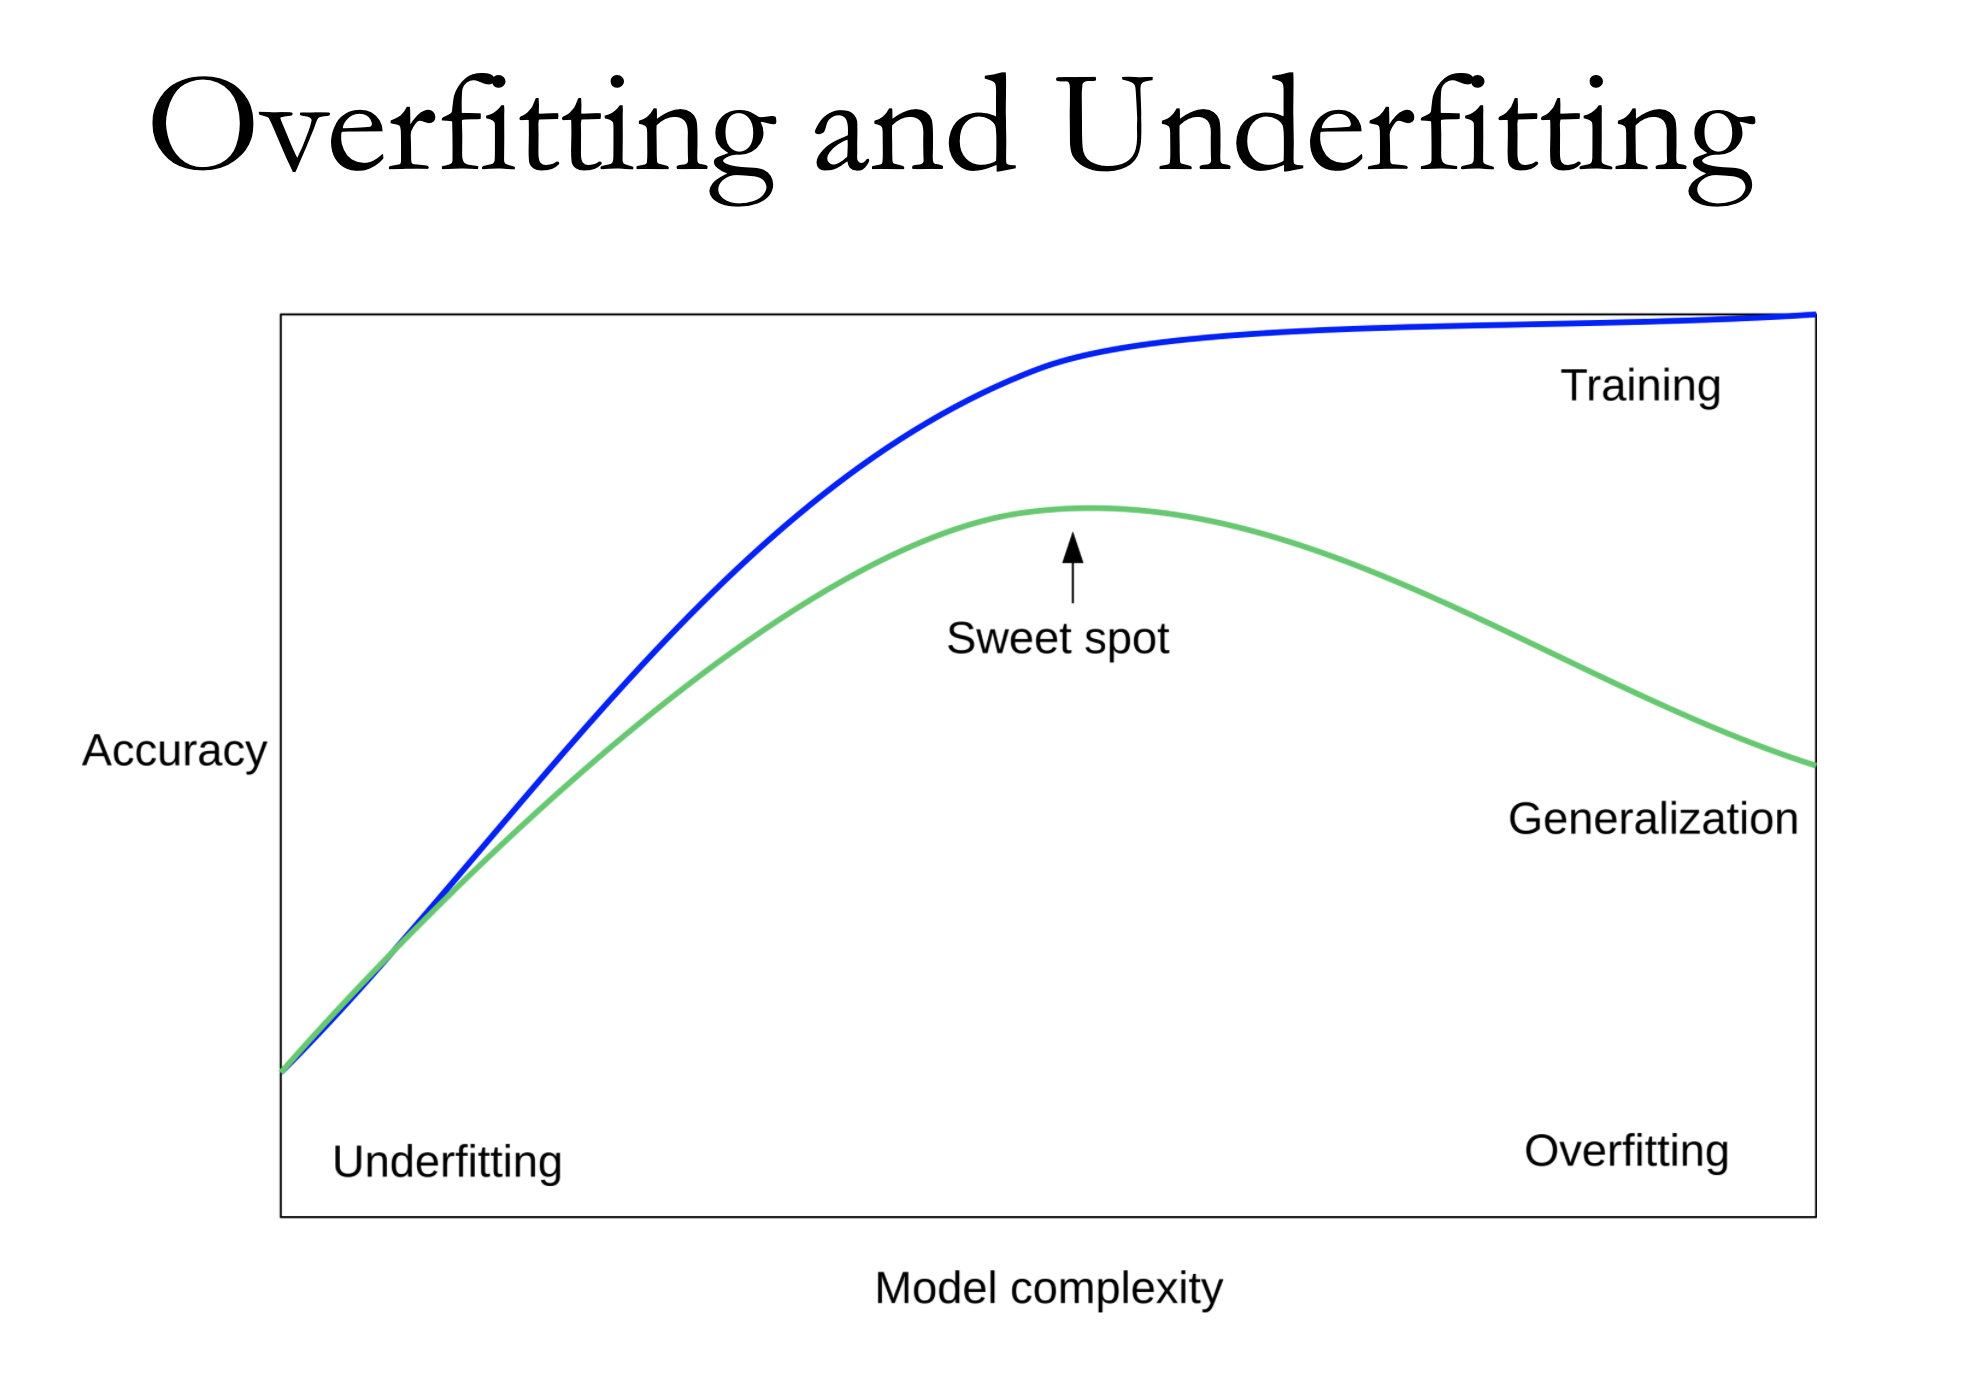
\includegraphics[width=0.9\linewidth ]{Figures/overfitting.png}
\end{figure}

\end{frame}




\begin{frame}
\frametitle{Questions}
\begin{itemize}

\item How are regularization techniques related with overfitting? 
\item What are the regularization techniques we have seen?
\item Why is it important to scale variables/features when performing regularization?

\end{itemize}
\end{frame}


\begin{frame}
\frametitle{We've seen }
\begin{figure}

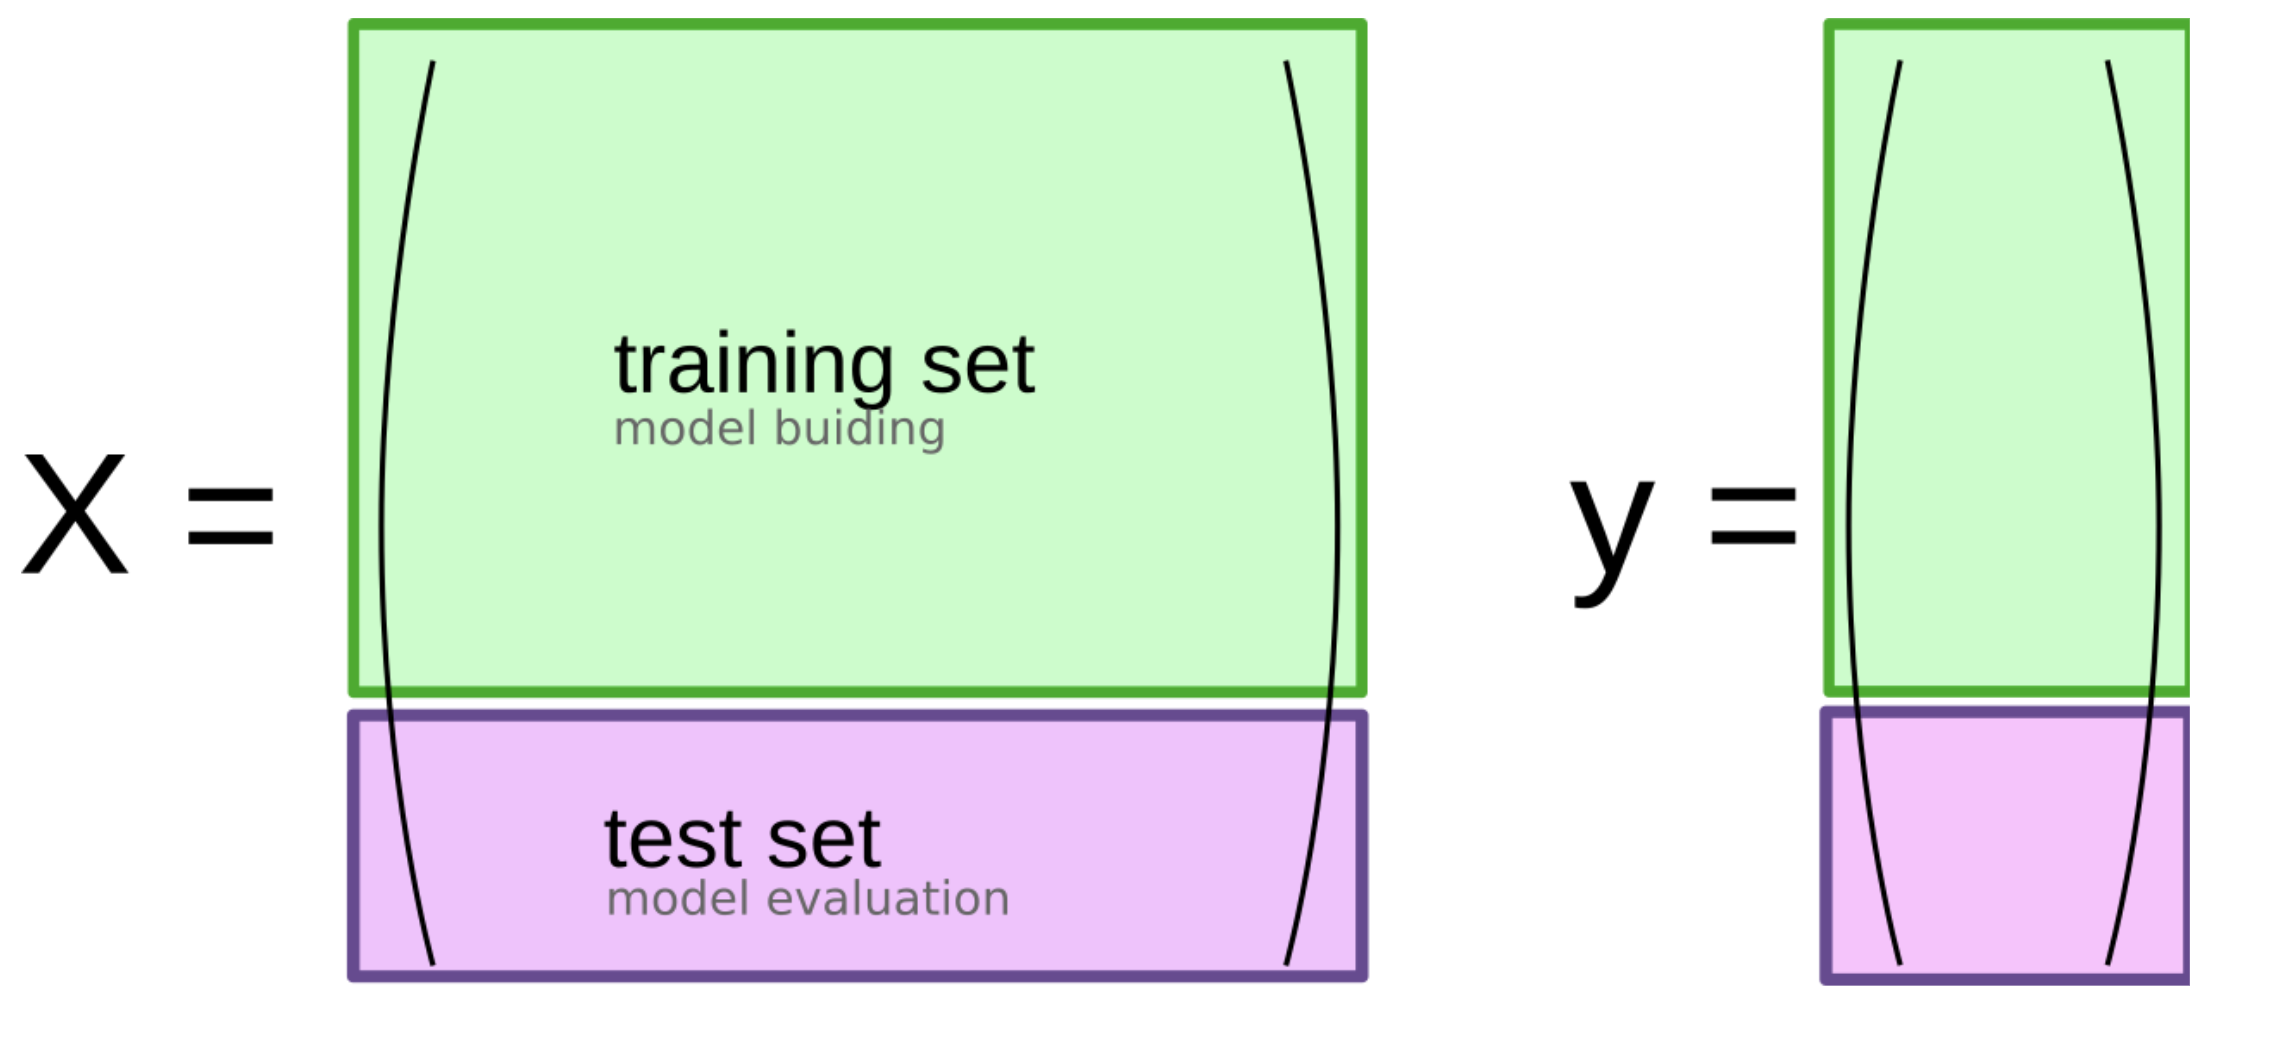
\includegraphics[width=0.9\linewidth ]{Figures/train-test-split.png}
\end{figure}

\end{frame}


\begin{frame}
\frametitle{We've seen}
\begin{figure}
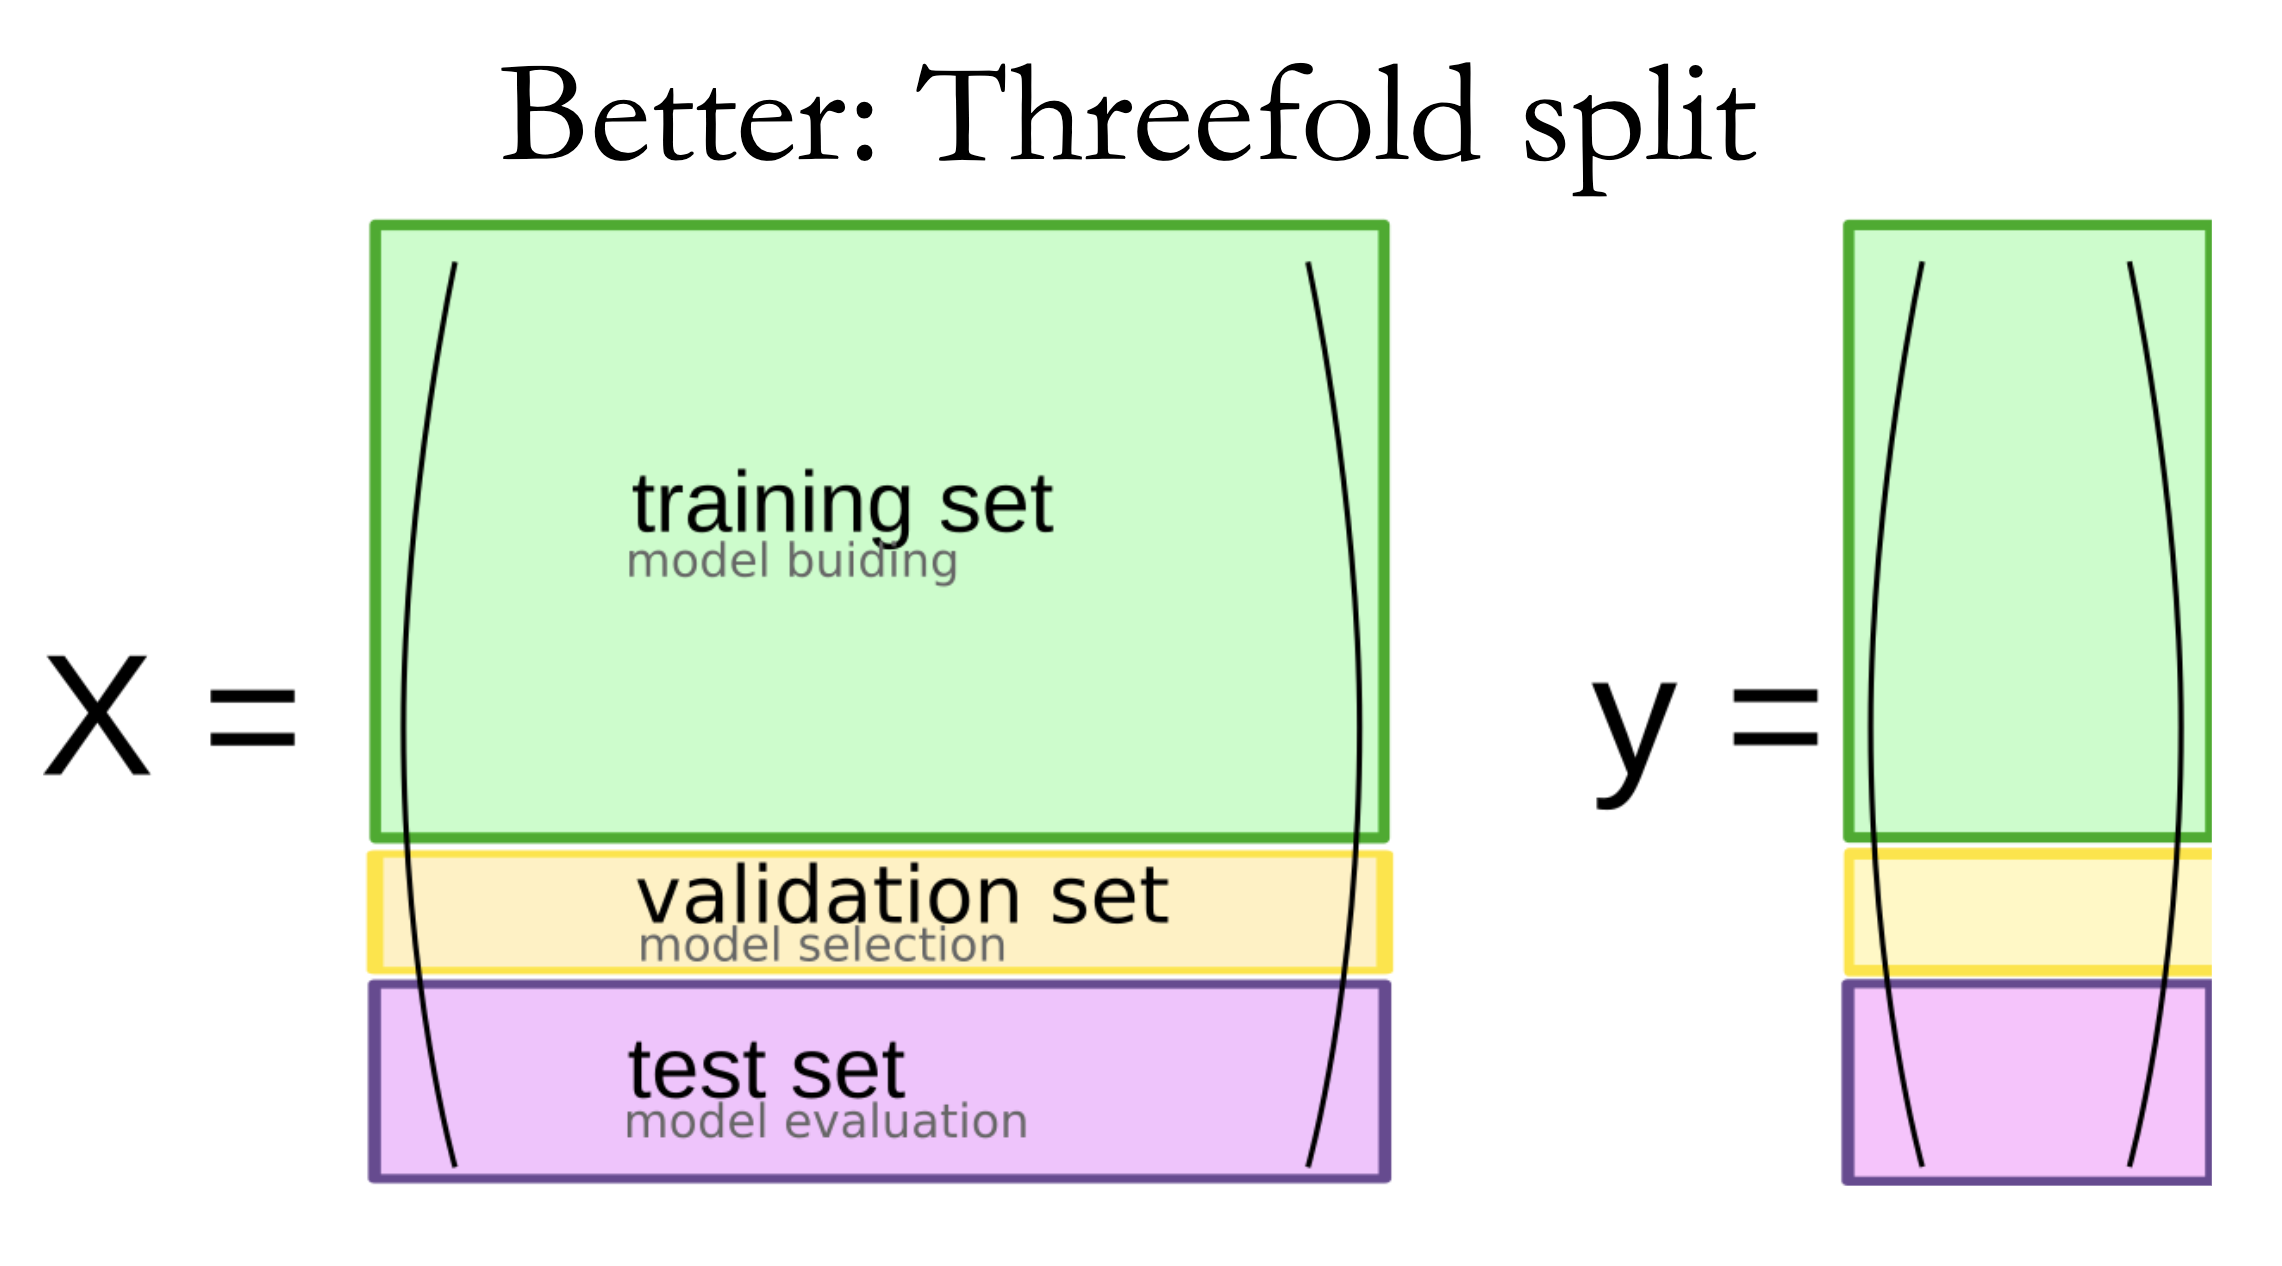
\includegraphics[width=0.9\linewidth ]{Figures/threefold-split.png}
\end{figure}
\end{frame}

\begin{frame}
\frametitle{We've seen}
\begin{figure}
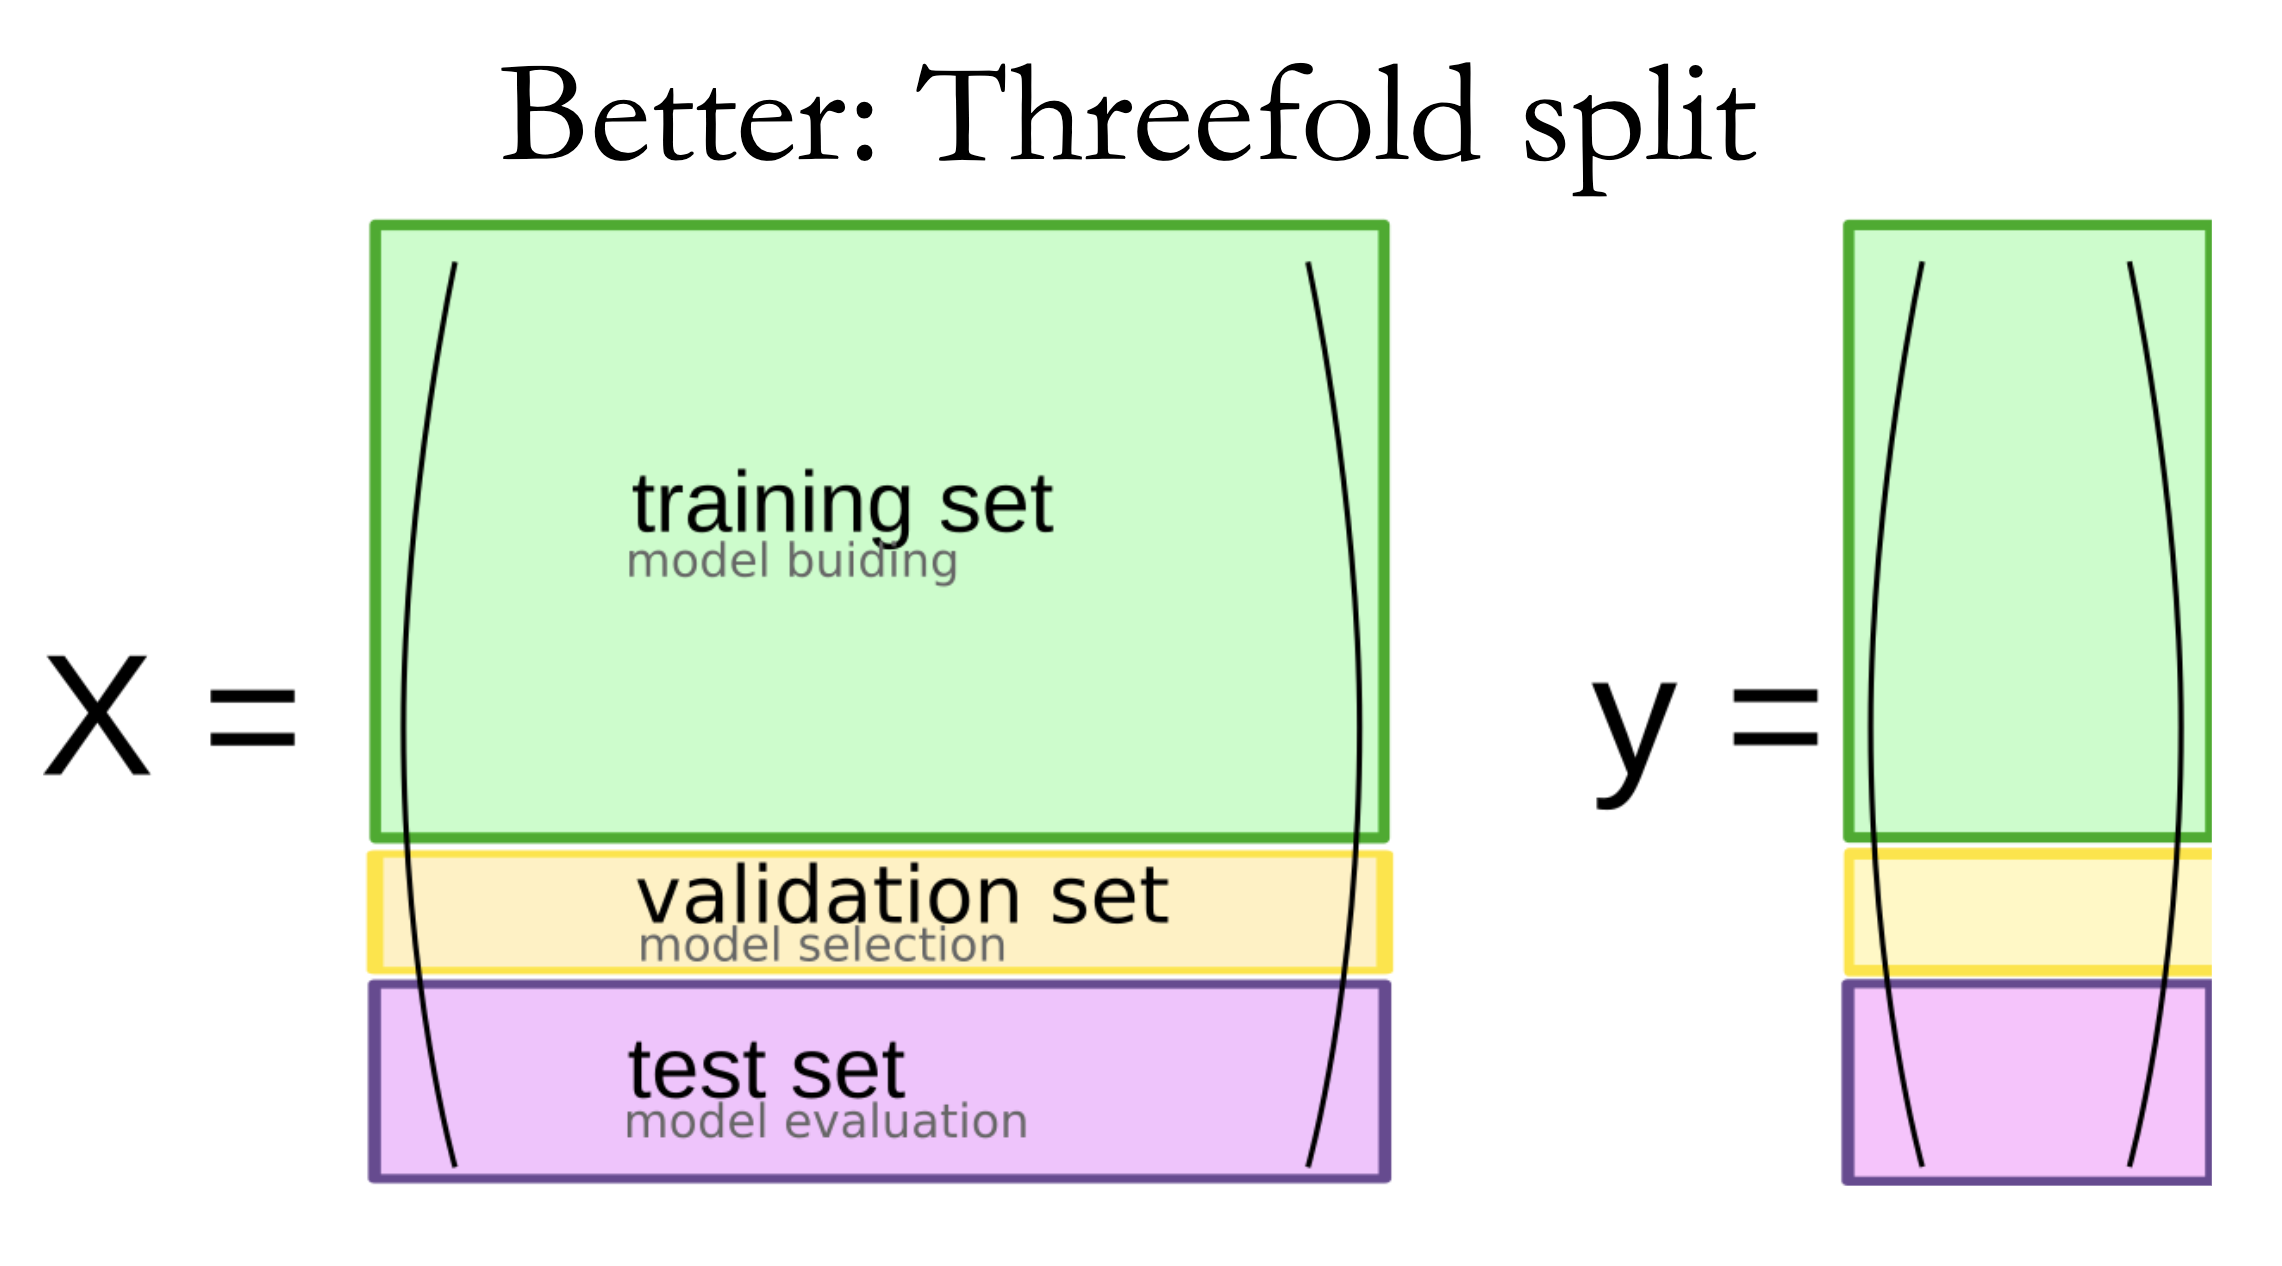
\includegraphics[width=0.9\linewidth ]{Figures/threefold-split.png}
\end{figure}
\end{frame}


\begin{frame}
\frametitle{Cross-Validation}
\begin{figure}
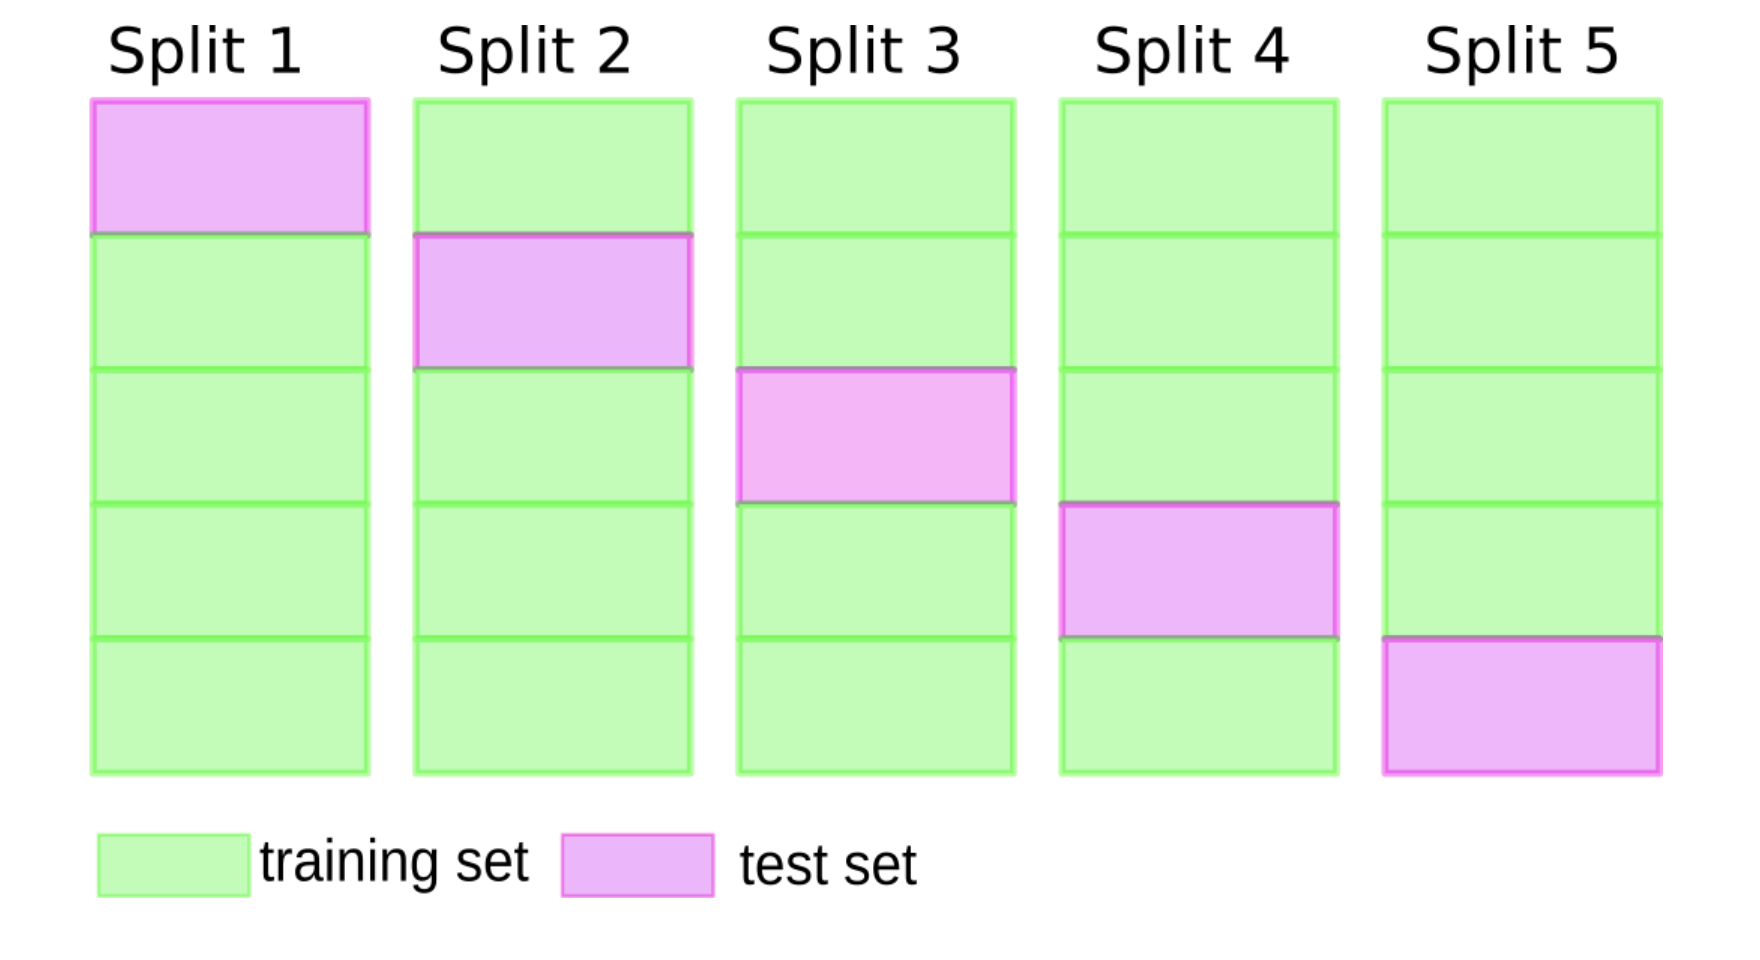
\includegraphics[width=0.9\linewidth ]{Figures/cv-5.png}
\end{figure}
\end{frame}


\begin{frame}
\frametitle{Cross-Validation}
\begin{figure}
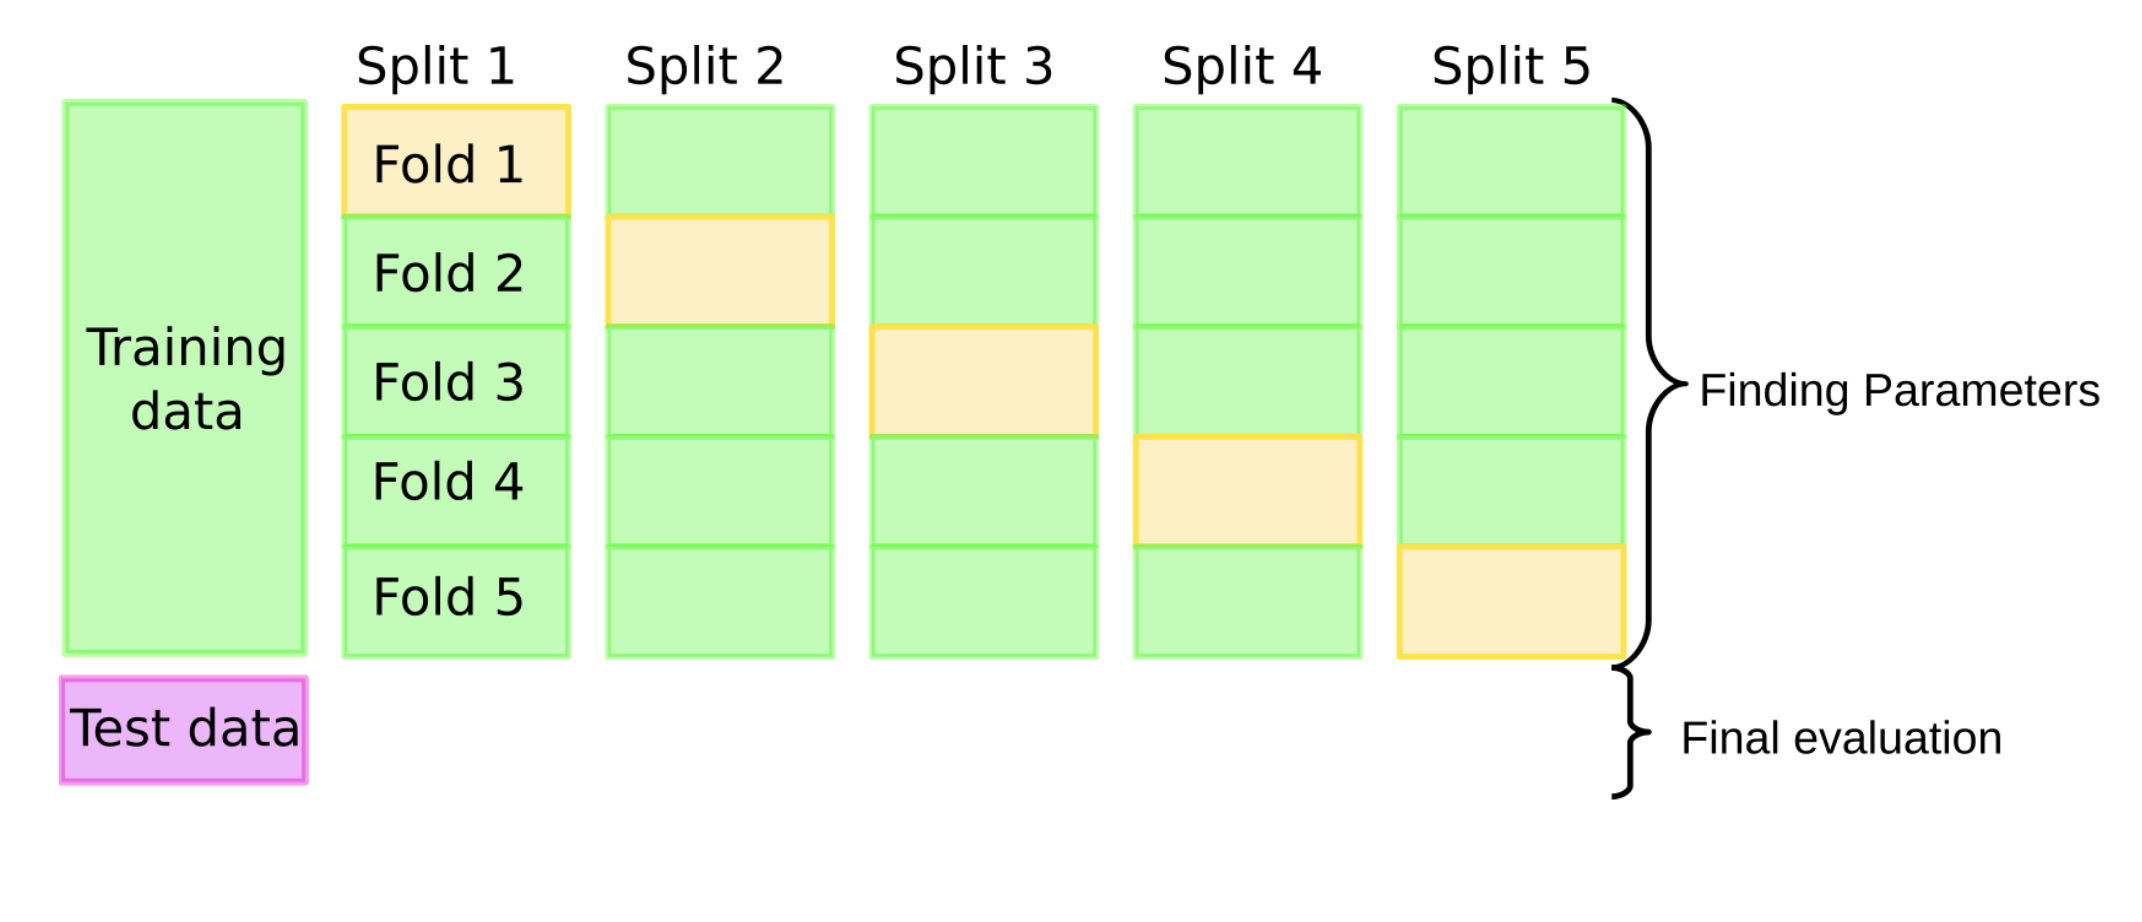
\includegraphics[width=\linewidth ]{Figures/cv-5-test.png}
\end{figure}
\end{frame}


\begin{frame}
\frametitle{Reminder!}
\begin{itemize}
\item Cross-validation
does not return a model
\item When calling cross\_val\_score, multiple models
are built internally, but the purpose of cross-validation is only to
evaluate how well a given algorithm will generalize when trained on a
specific dataset
\end{itemize}
\end{frame}


 



\begin{frame}
\begin{center}
\Large{\textbf{Cross-Validation Strategies }}
\end{center}
\end{frame}


\begin{frame}
\begin{figure}
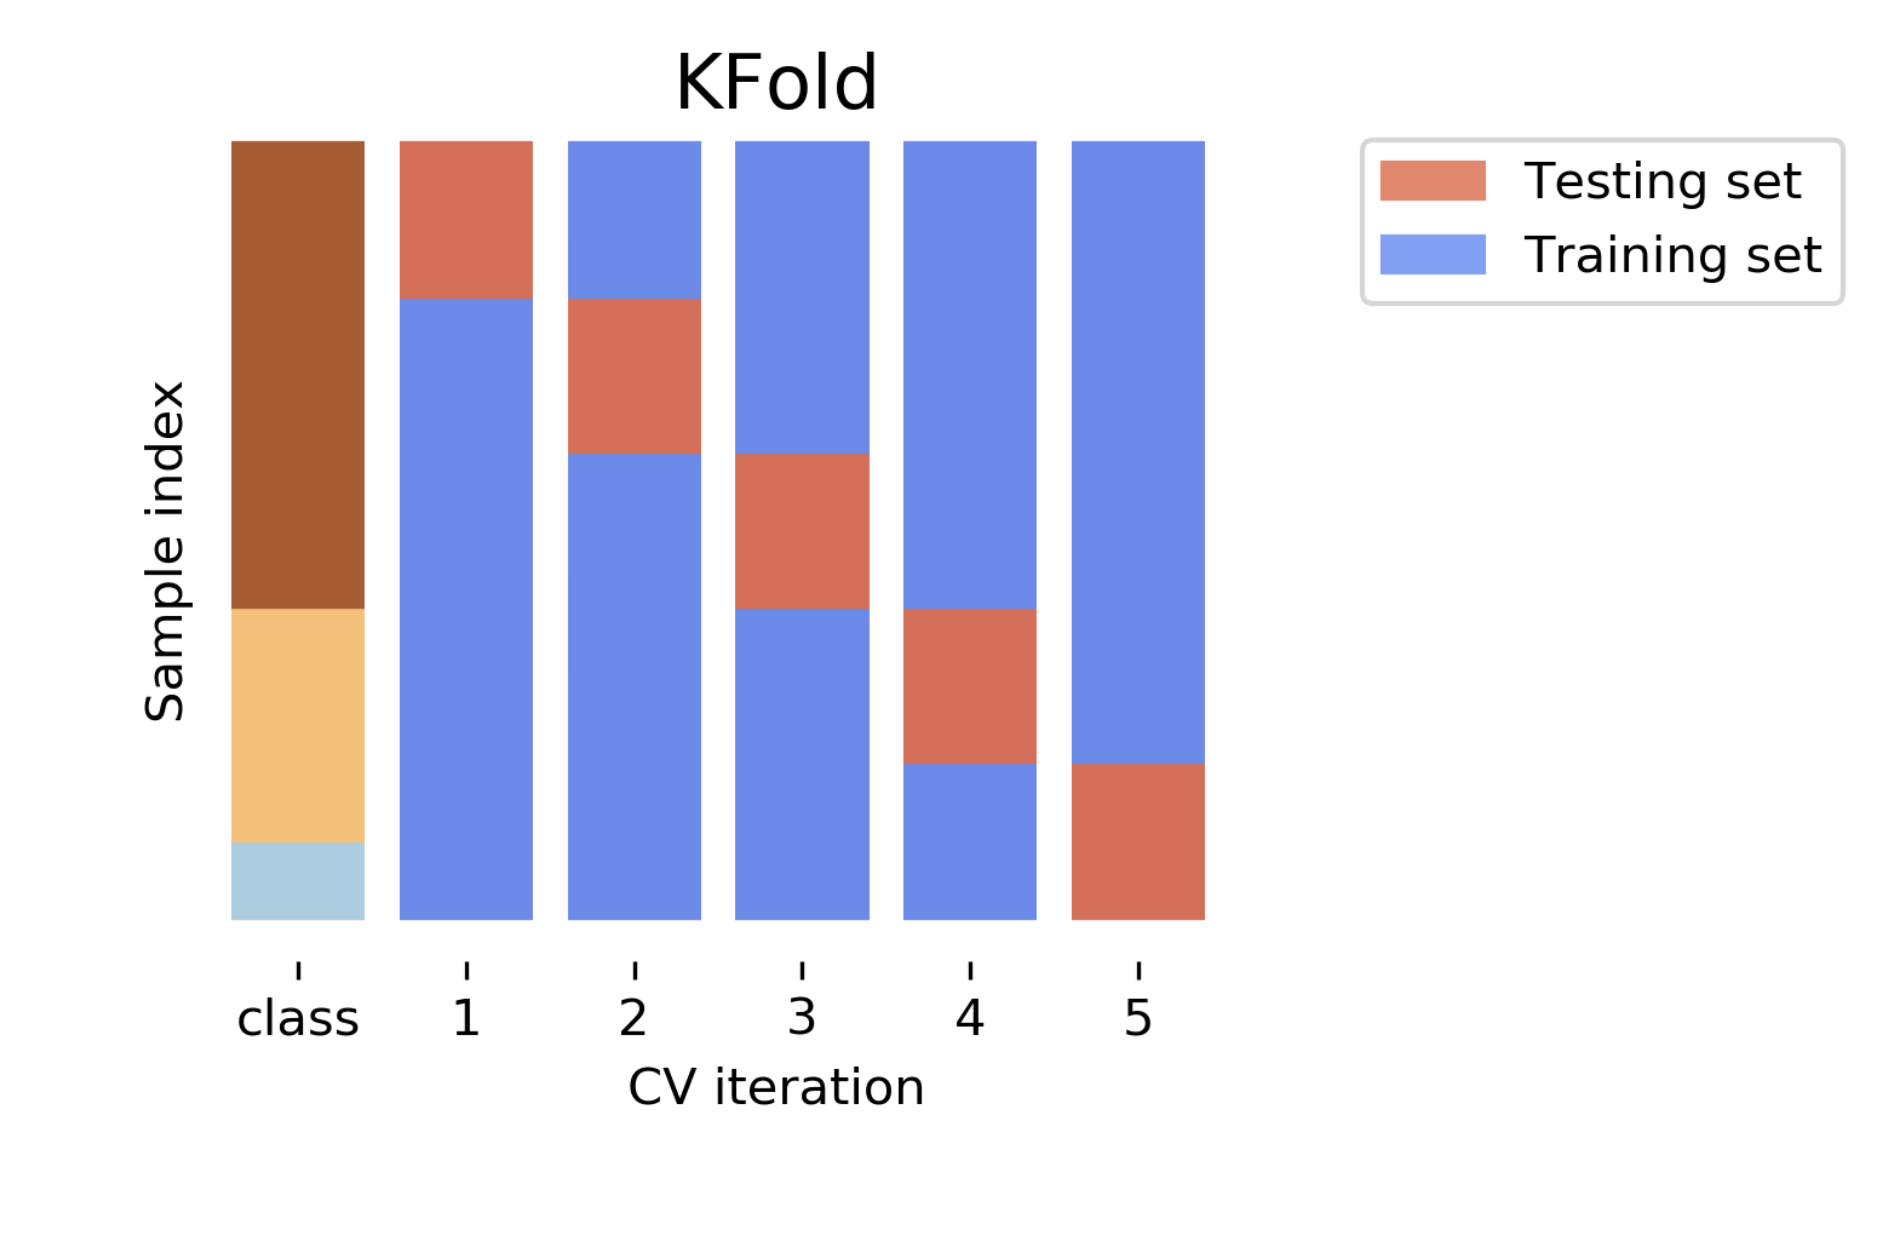
\includegraphics[width=\linewidth ]{Figures/k-fold.png}
\end{figure}
\end{frame}

\begin{frame}
\begin{figure}
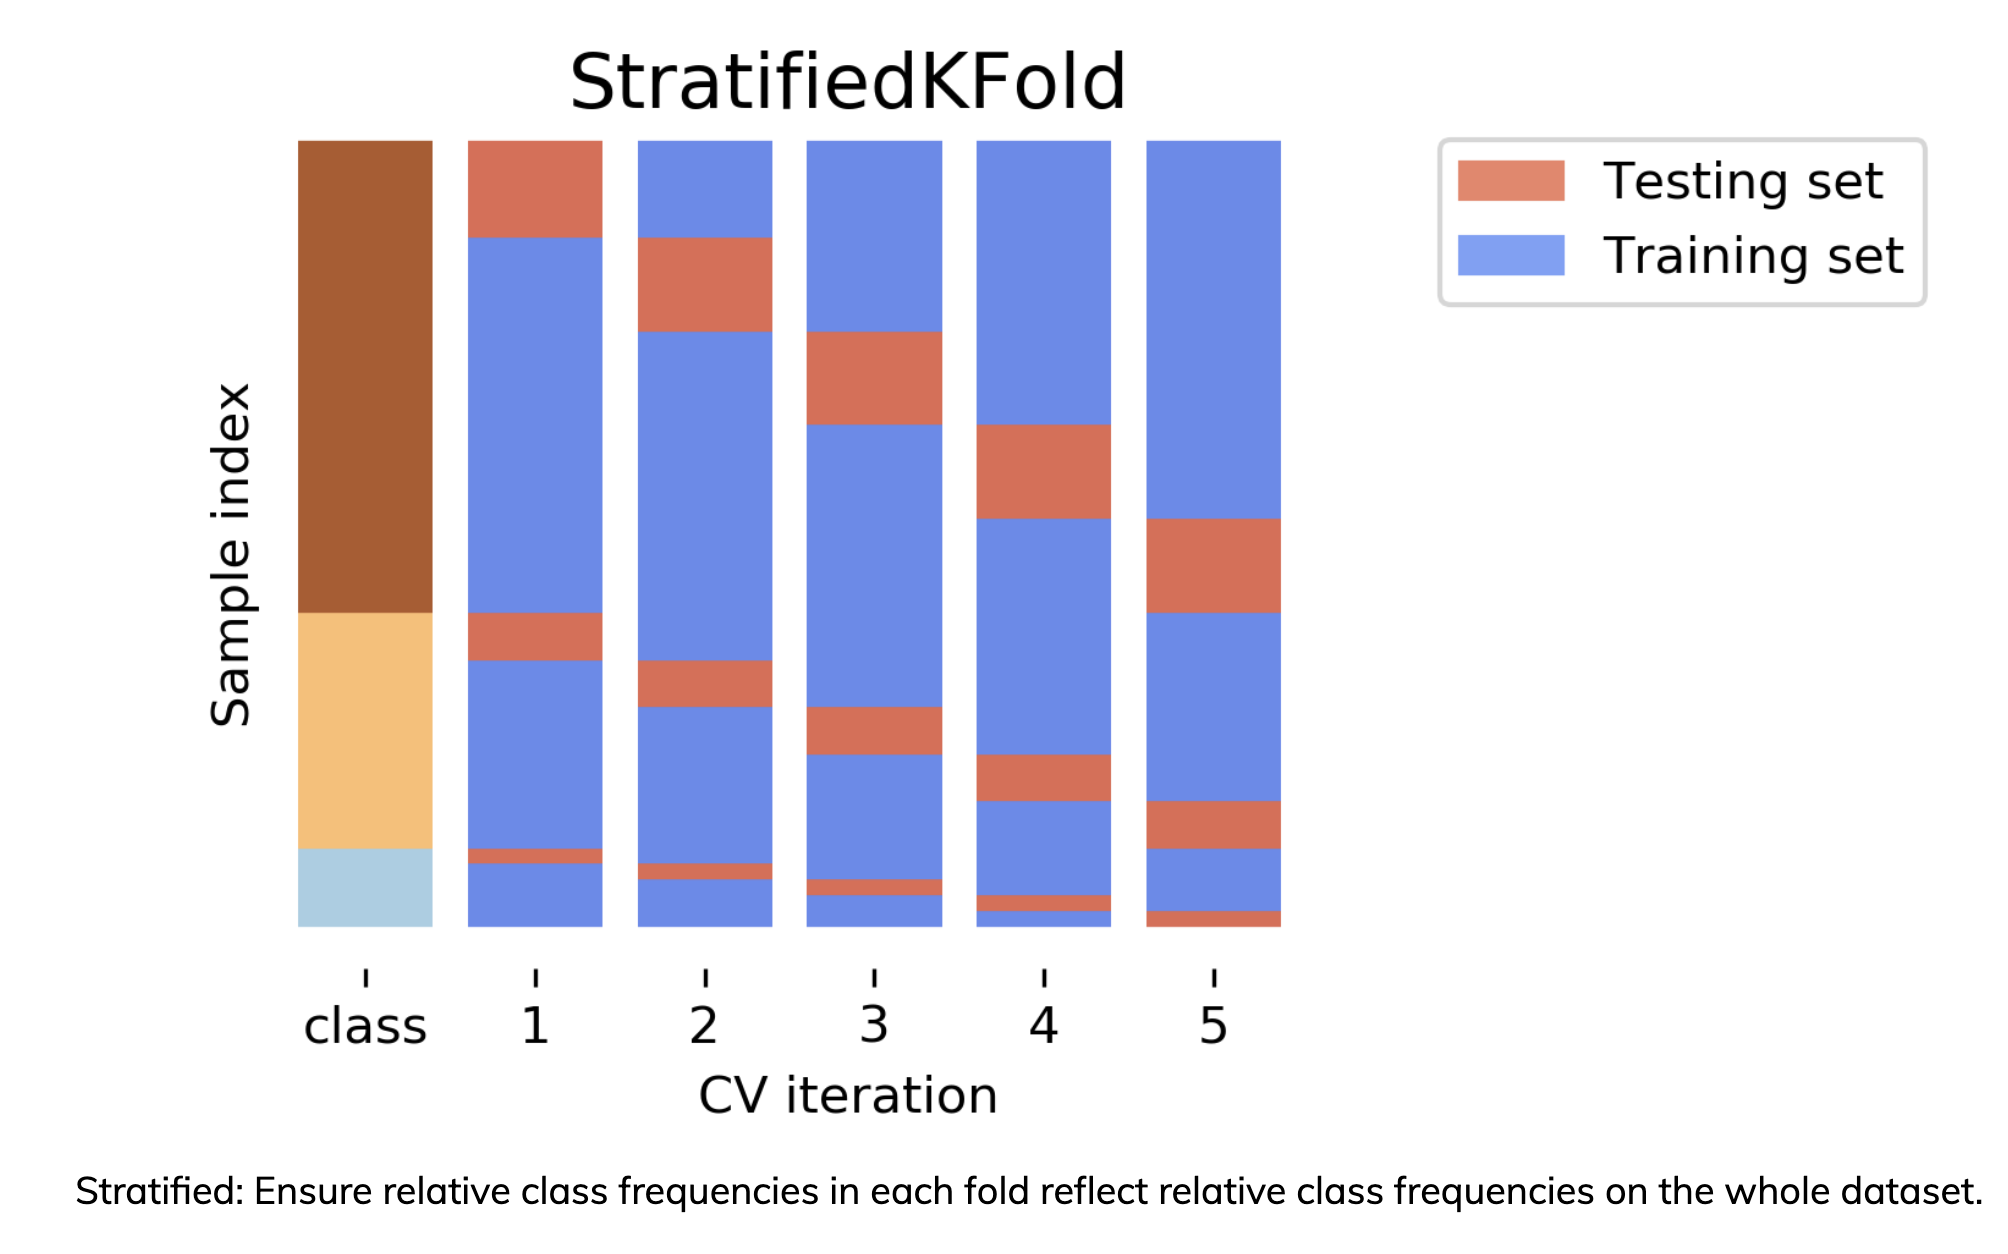
\includegraphics[width=\linewidth ]{Figures/stratified-k-fold.png}
\end{figure}
\end{frame}



\begin{frame}
\frametitle{Why stratifying?}
\begin{itemize}
\item Assume a (multi-class) classification problem. What happens if a class not stratified by chance?
\end{itemize}
\end{frame}



\begin{frame}
\frametitle{Repeated K-Fold and Leave-One-Out}
\begin{itemize}

\item Leave-One-Out: K-Fold (number of folds equals number of observations)
	\begin{itemize}
	\item Drawback: High variance, takes a long time
	\end{itemize}

\item Better: Shuffle Split (Monte Carlo)
	\begin{itemize}
	\item Repeatedly sample a test set with replacement
	\end{itemize}

\item Even Better: Repeated K-Fold
	\begin{itemize}
	\item Apply K-Fold or Stratified K-Fold multiple times with shuffled data
	\end{itemize}

\end{itemize}
\end{frame}



\begin{frame}
\begin{figure}
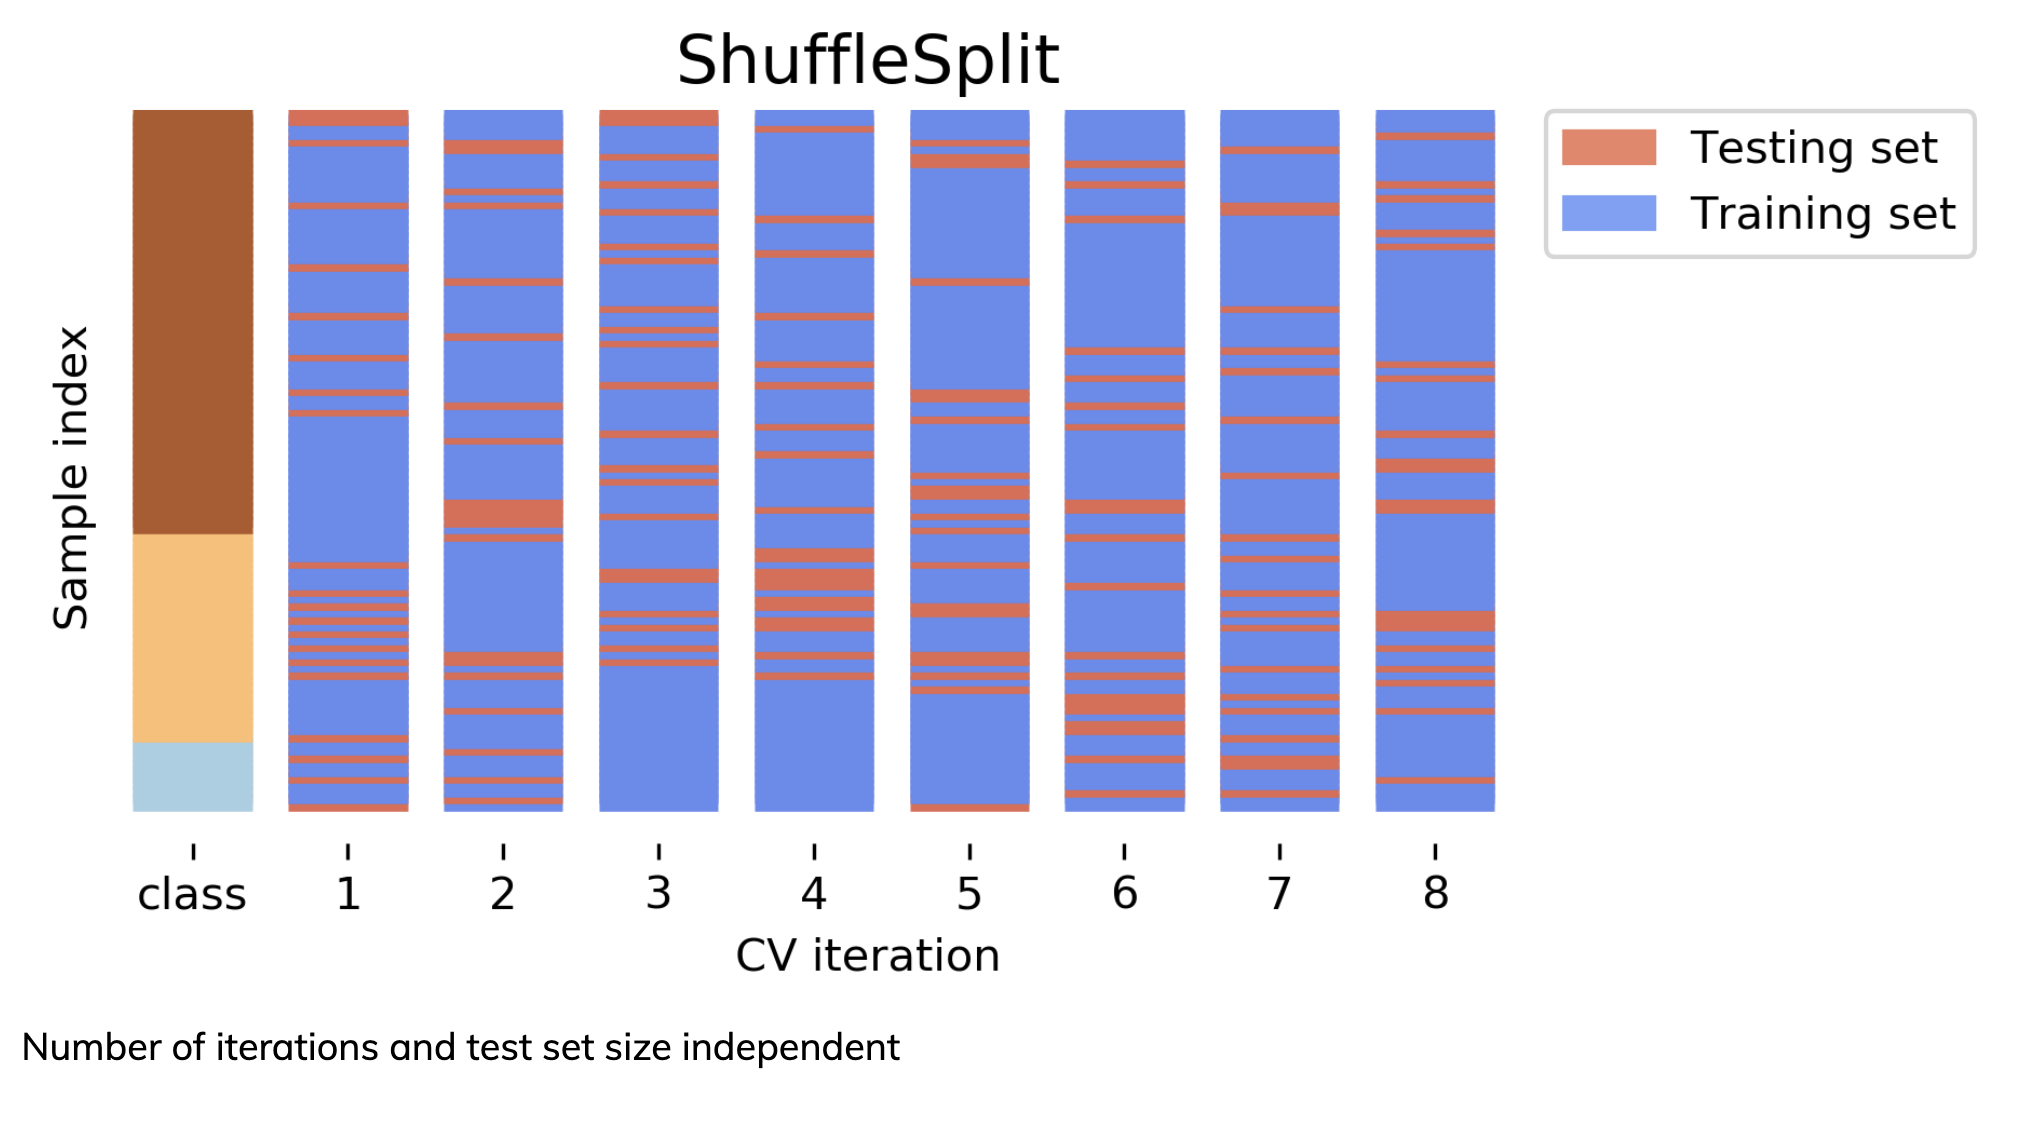
\includegraphics[width=\linewidth ]{Figures/shuffle-split.png}
\end{figure}
\end{frame}



\begin{frame}
\frametitle{Defaults in scikit-learn}
\begin{itemize}
\item 5-fold in 0.22 (used to be 3 fold)
\item For classification cross-validation is stratified
\item train\_test\_split has stratify option: train\_test\_split(X, y, stratify=y)
\item No shuffle by default!
\end{itemize}
\end{frame}


\begin{frame}
\begin{center}
\Large{\textbf{Cross-Validation for correlated data}}
\end{center}
\end{frame}


\begin{frame}
\frametitle{Cross-Validation non-iid data}
Know your data and setting
\begin{itemize}
\item Time-series data have a time component 
\item Geographical data have a spatial component
\item Grouped data
\item DON'T SHUFFLE if dealing with any of the above. Why?
\end{itemize}
\end{frame}


\begin{frame}
\begin{figure}
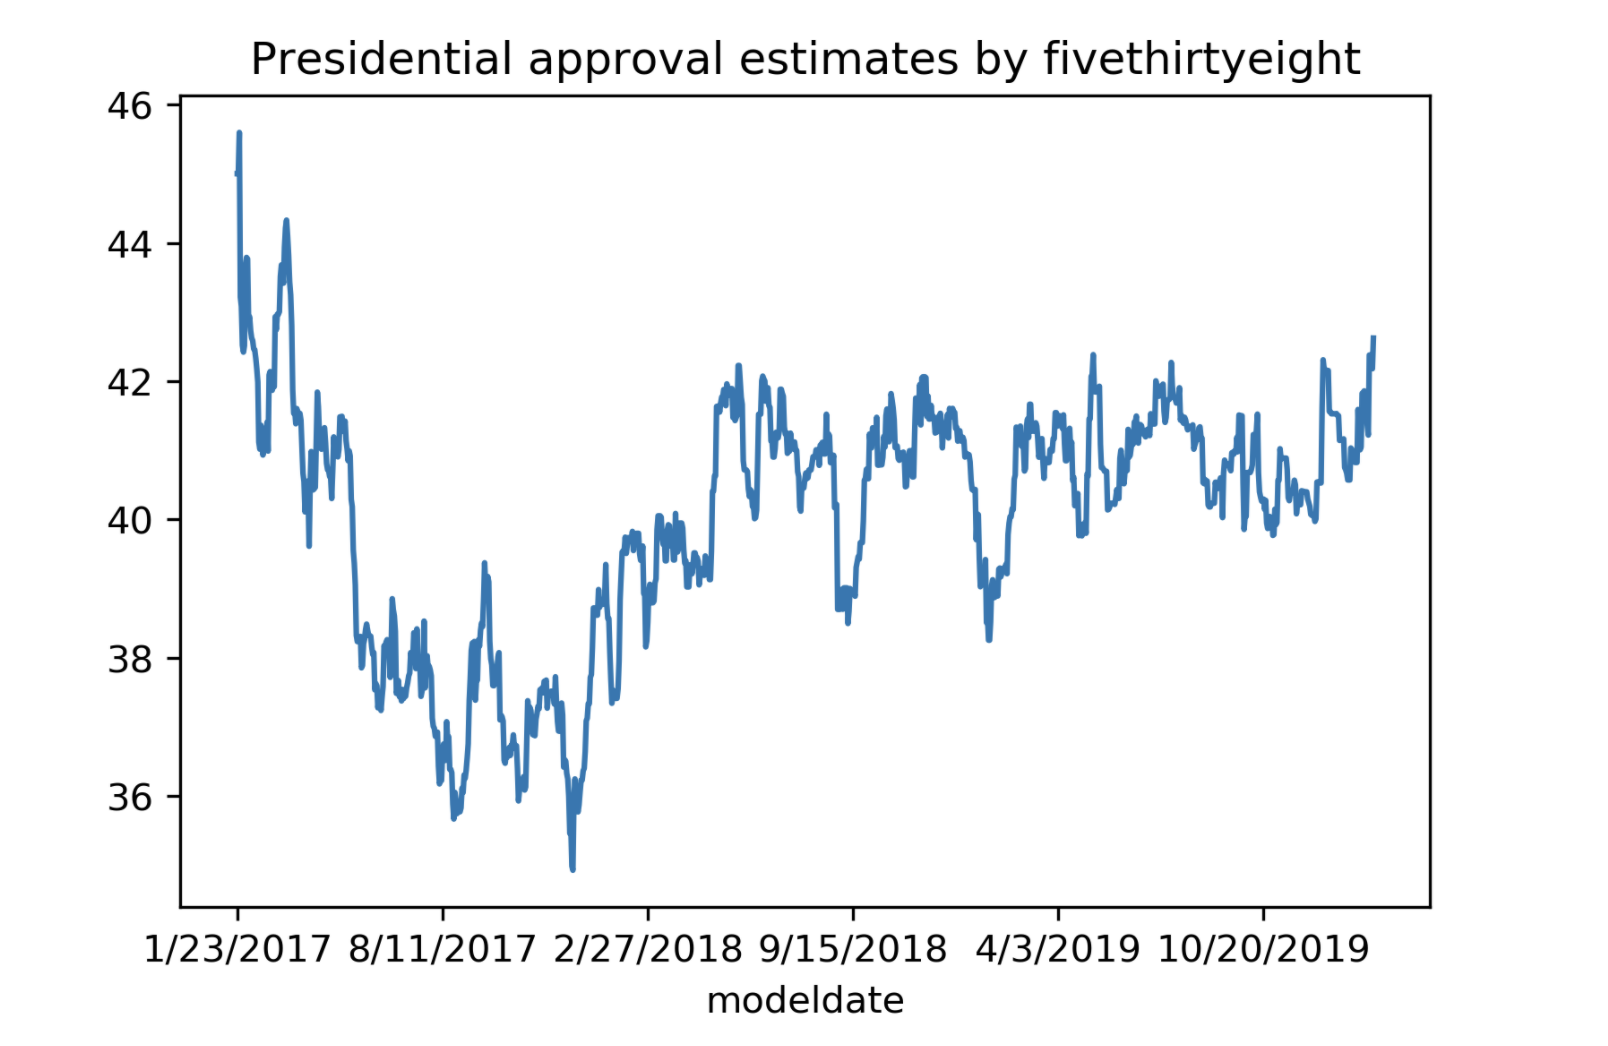
\includegraphics[width=\linewidth ]{Figures/time-series.png}
\end{figure}
\end{frame}

\begin{frame}
\begin{figure}
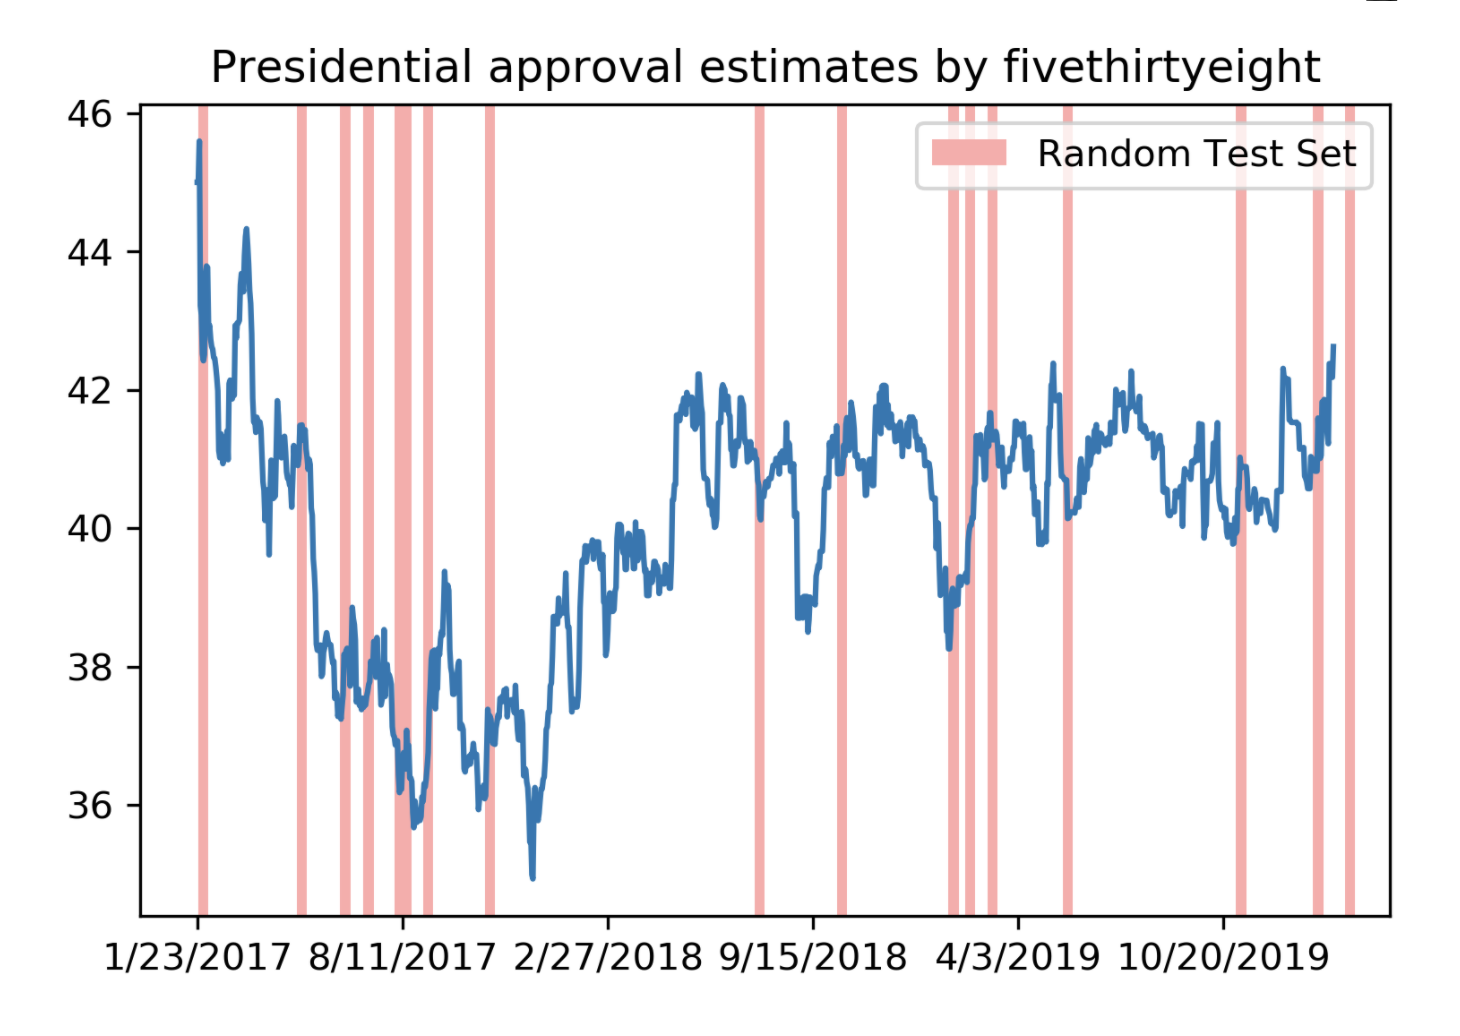
\includegraphics[width=\linewidth ]{Figures/time-series-split.png}
\end{figure}
\end{frame}

\begin{frame}
\begin{figure}
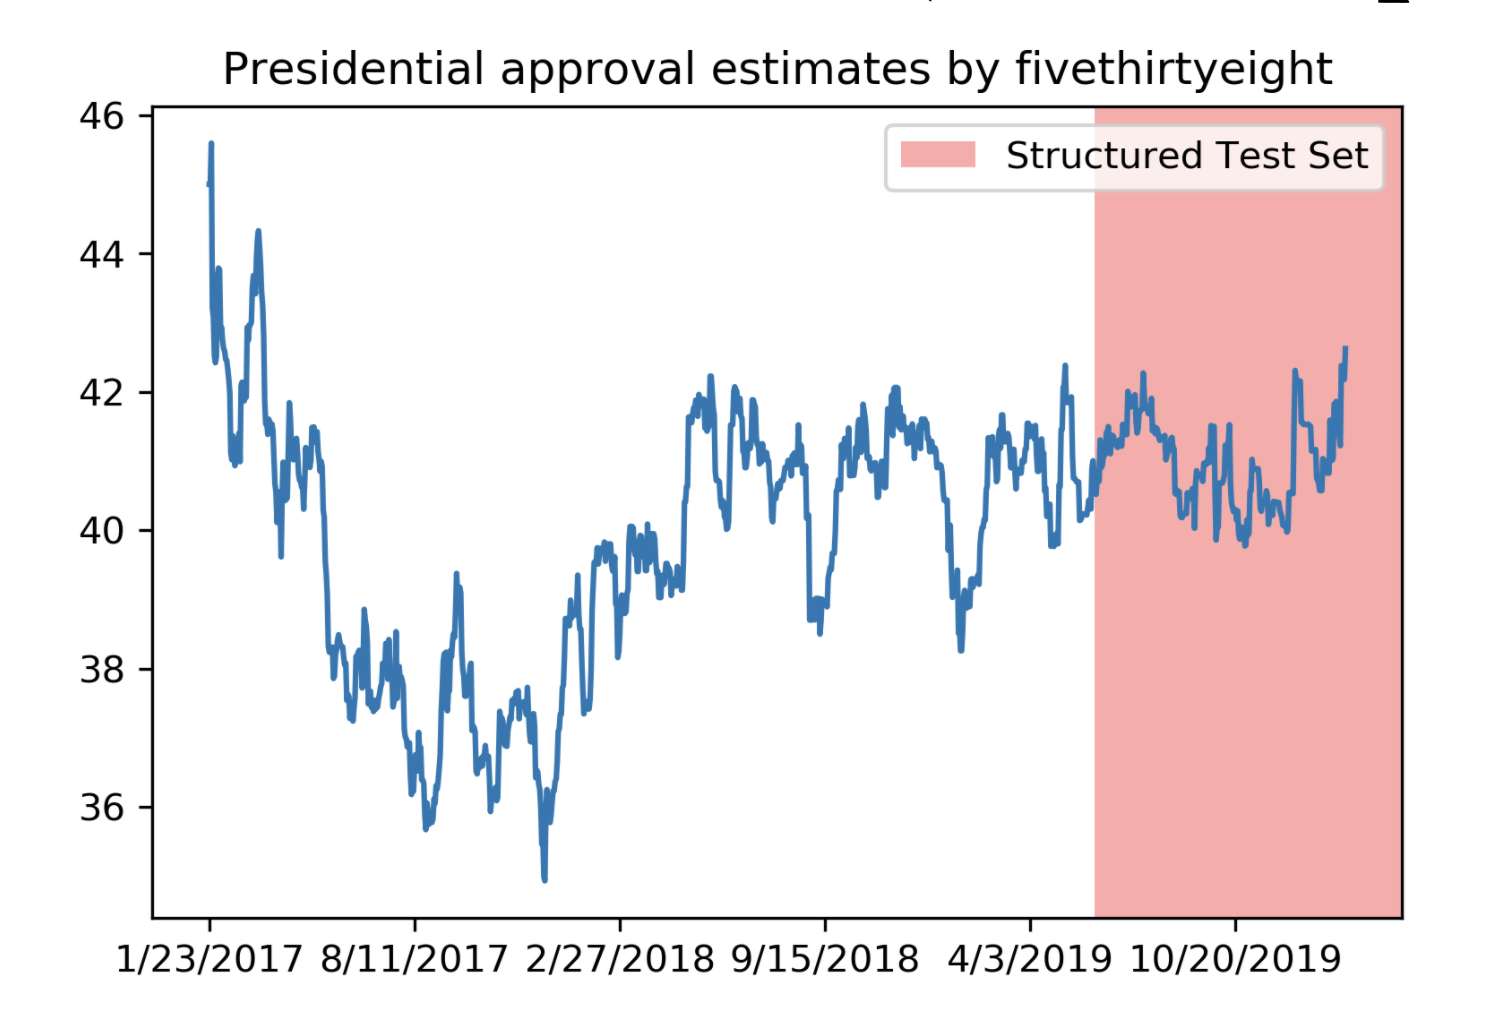
\includegraphics[width=\linewidth ]{Figures/time-series-train-test.png}
\end{figure}
\end{frame}

\begin{frame}
\begin{figure}
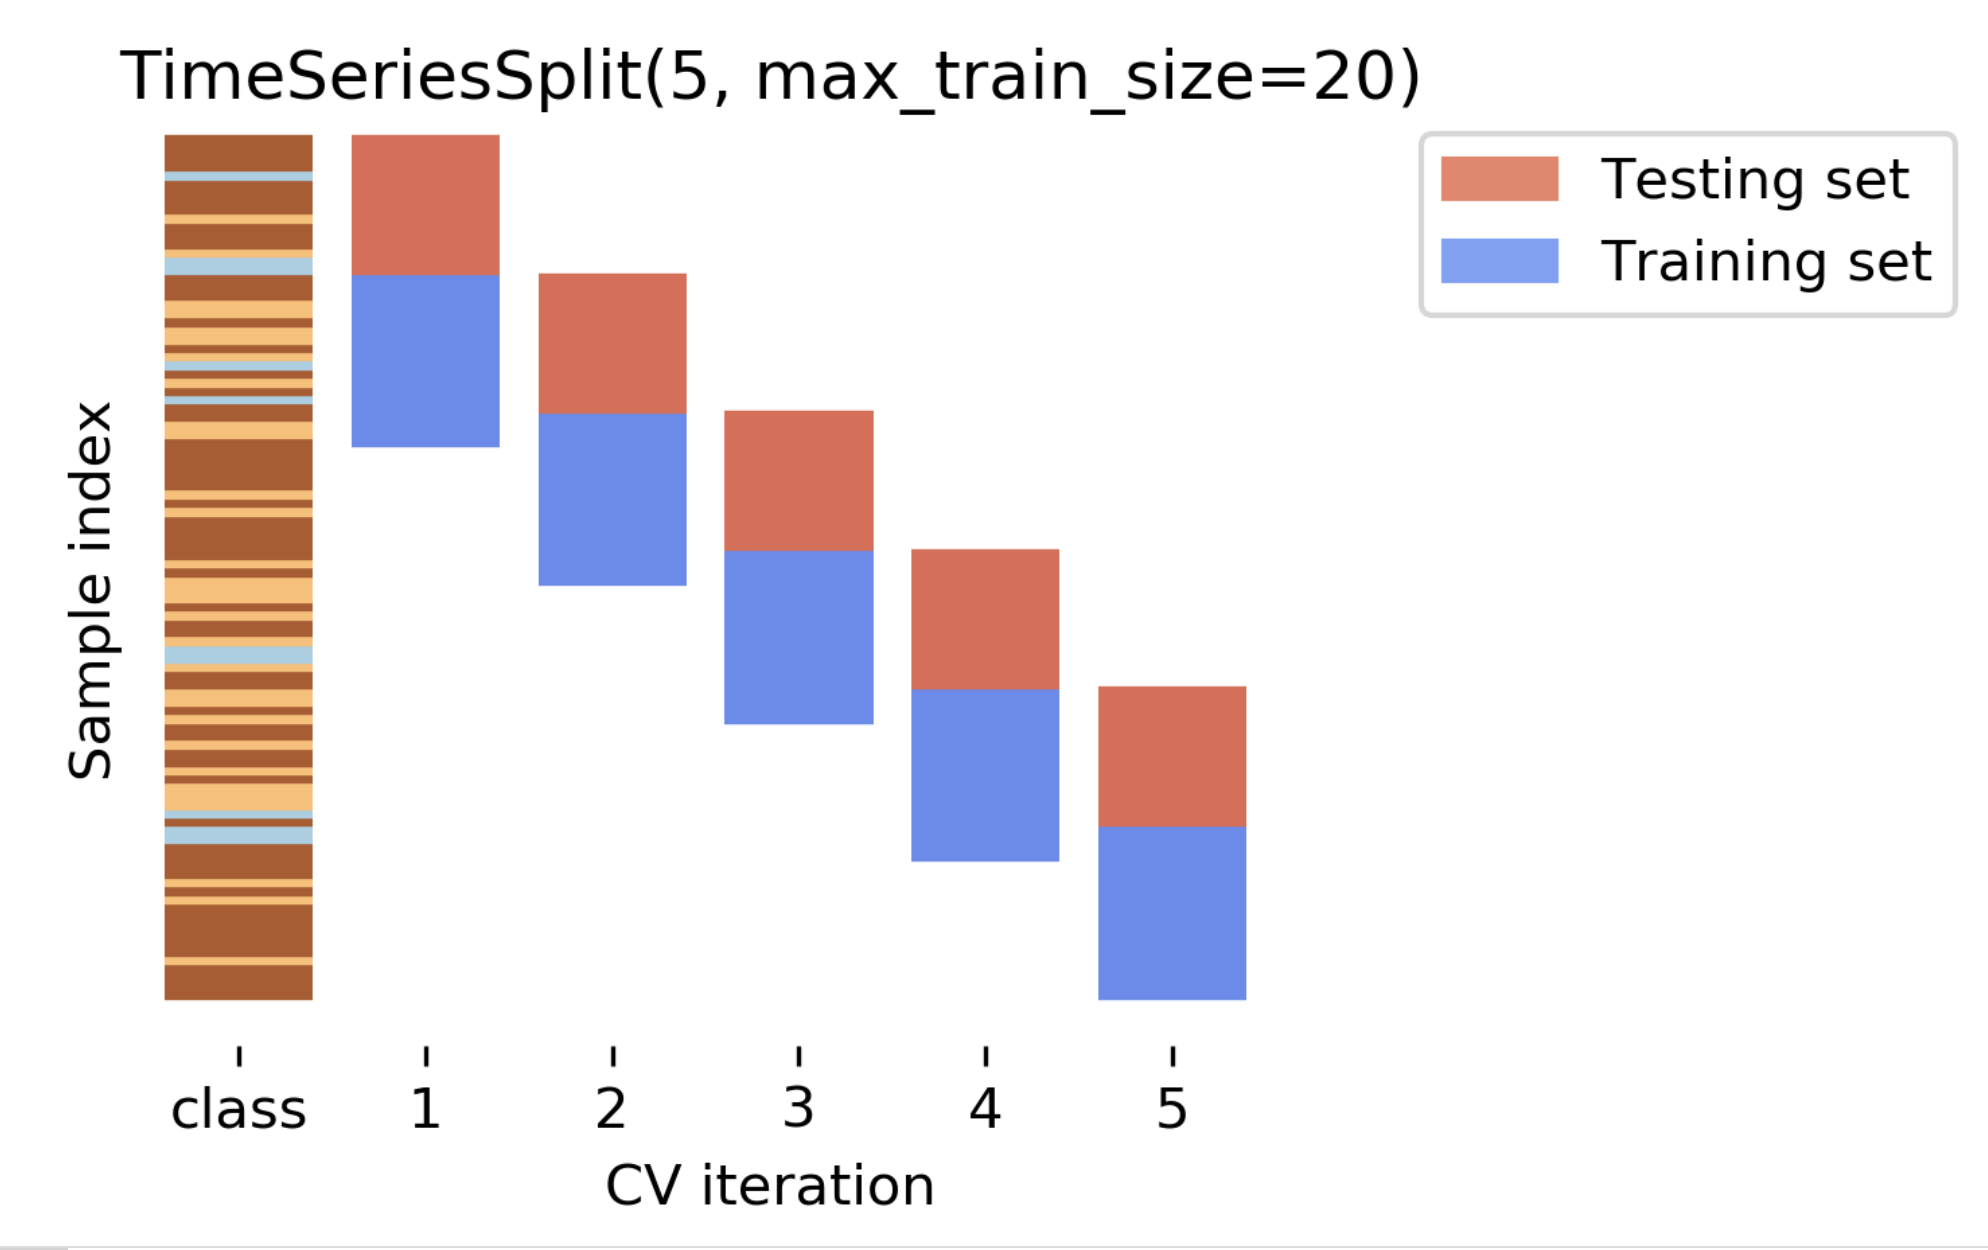
\includegraphics[width=\linewidth ]{Figures/time-series-rolling.png}
\end{figure}
\end{frame}


\begin{frame}
\begin{figure}
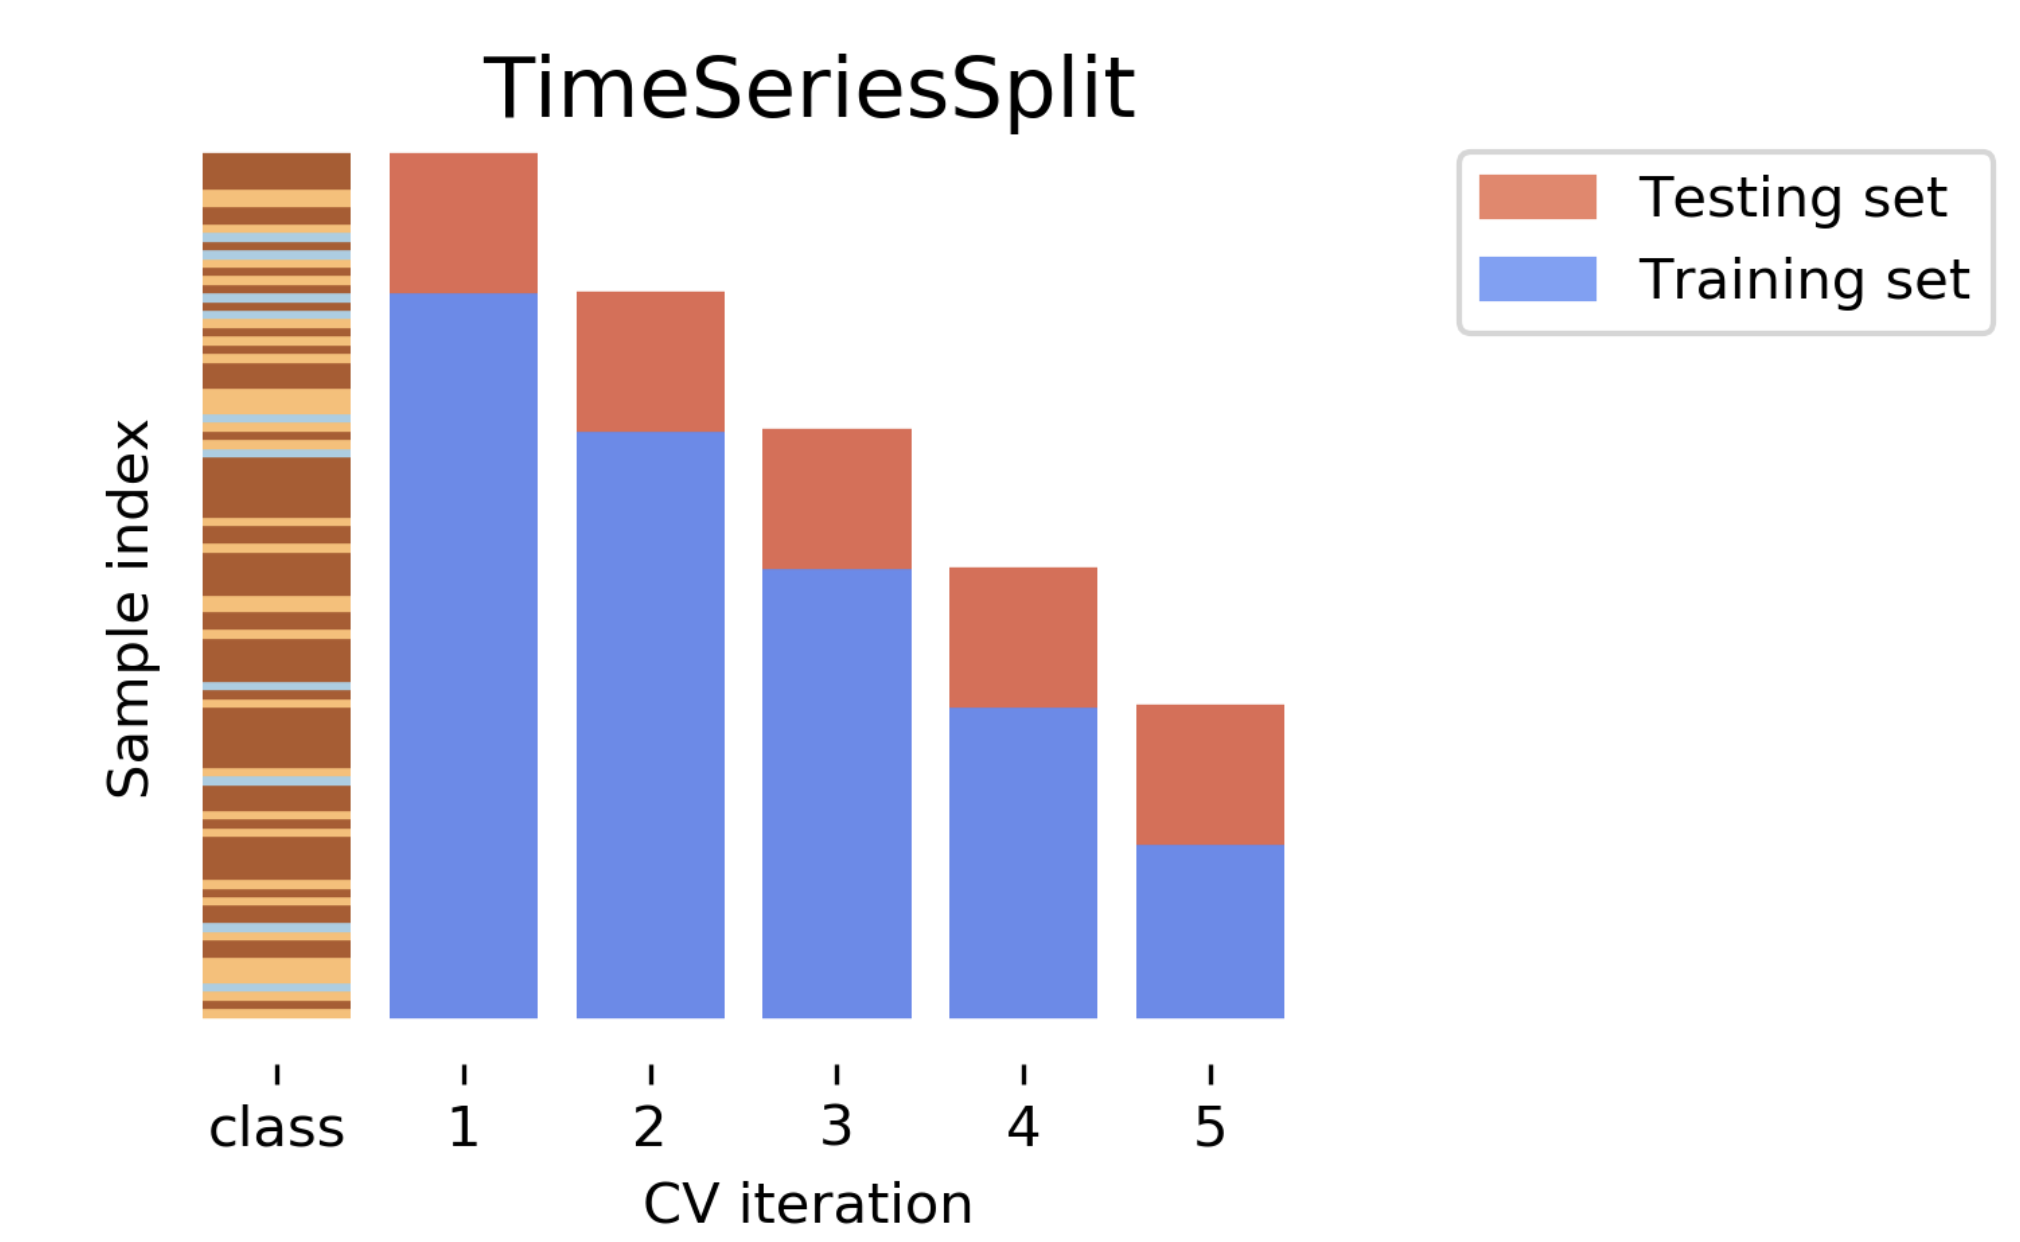
\includegraphics[width=\linewidth ]{Figures/time-series-rolling2.png}
\end{figure}
\end{frame}


\begin{frame}
\begin{center}
\Large{\textbf{Model Interpretation and Feature Selection}}
\end{center}
\end{frame}

\begin{frame}
\frametitle{Model Interpretation}
Black-box
\begin{itemize}
\item No inference
\item No causality
\item Still useful
\end{itemize}
\end{frame}


\begin{frame}
\frametitle{Types of explanations}
Explain model globally

\begin{itemize}
	\item How does the output depend on the input?
	\item Often: some form of marginals
\end{itemize}

Explain model locally
\begin{itemize}
	\item Why did it classify this point this way?

	\item Explanation could look like a "global" one but be different for each point
	\item What is the minimum change to classify it differently?
	\end{itemize}
\end{frame}


\begin{frame}
\frametitle{explain model $\neq$ explain data}
Explain model globally

\begin{itemize}
\item Model inspection only tells you about the model

\item The model might not accurately reflect the data

\end{itemize}
\end{frame}



\begin{frame}
\frametitle{Features important to the model}
Naive:
\begin{itemize}
	\item coef\_ for linear models


	\item feature\_importances\_ for tree-based models

\end{itemize}
Use with care!
\end{frame}


\begin{frame}
\frametitle{Linear Model coefficients}
\begin{itemize}
\item Relative importance only meaningful after scaling
\item Correlation among features might make coefficients completely uninterpretable

\item $L1$ regularization will pick one at random from a correlated group (try this in the regularization notebook)!
\item Any penalty will invalidate usual interpretation of linear coefficients

\end{itemize}
\end{frame}

\end{document}


